\RequirePackage{fix-cm}
\documentclass{beamer}
\usetheme{Boadilla}
\usecolortheme{seahorse}
\usefonttheme{serif}

\usepackage{graphicx,xcolor}
\usepackage{amsmath,amssymb,amsfonts,booktabs}
\usepackage{tikz,pgfplots}
\usetikzlibrary{arrows.meta,positioning}
\usepgfplotslibrary{groupplots,fillbetween}
\pgfplotsset{compat=1.18}

\definecolor{eegteal}{HTML}{267C72}
\definecolor{eegcoral}{HTML}{C2603B}
\definecolor{eegblue}{HTML}{4968B1}
\definecolor{muted}{HTML}{526071}
\setbeamertemplate{navigation symbols}{}
% Retain the Boadilla footer's title/date/page areas without its author block.
\setbeamertemplate{footline}{%
  \leavevmode\hbox{%
    \begin{beamercolorbox}[wd=.333333\paperwidth,ht=2.25ex,dp=1ex]{author in head/foot}
    \end{beamercolorbox}%
    \begin{beamercolorbox}[wd=.333333\paperwidth,ht=2.25ex,dp=1ex,center]{title in head/foot}
      \usebeamerfont{title in head/foot}\insertshorttitle
    \end{beamercolorbox}%
    \begin{beamercolorbox}[wd=.333333\paperwidth,ht=2.25ex,dp=1ex,right]{date in head/foot}
      \usebeamerfont{date in head/foot}\insertshortdate{}\hspace*{2em}
      \insertframenumber{} / \inserttotalframenumber\hspace*{2ex}
    \end{beamercolorbox}%
  }\vskip0pt
}
\setbeamercolor{alerted text}{fg=eegteal}
\setbeamerfont{frametitle}{size=\Large}
\hypersetup{colorlinks=true,urlcolor=eegblue,linkcolor=black,citecolor=eegblue}

\title[EEG Compression]{EEG Compression}
\subtitle{Multi Modal Data Processing and Learning}
\author[D. Das / 240150049]{\texorpdfstring{Debarghya Das\\240150049}{Debarghya Das (240150049)}}
\institute[DSAI, IITG]{Mehta Family School of Data Science and Artificial Intelligence\\
Indian Institute of Technology, Guwahati}
\date{25 November 2026}
\titlegraphic{
\includegraphics[width=2cm]{images/logo/IITG.jpg}}

% Keep Beamer's default 4:3 canvas and the supplied theme. The requested
% title frame precedes twelve content slides. No outline frames are inserted.
\setbeameroption{hide notes}
\newcommand{\credit}[1]{\vfill{\raggedright\fontsize{6.5}{8}\selectfont\color{muted}#1\par}}
\newcommand{\smalltext}[1]{{\fontsize{8}{10}\selectfont #1\par}}
\newcommand{\refentry}[3]{\textbf{#1}\\\href{#3}{#2}\par\vspace{0.6em}}
\newcommand{\taskcurve}[3]{%
  \addplot[name path=#3-#1-low,draw=none,forget plot]
    table[x=budget,y=#1lo,col sep=comma]{data/#3.csv};
  \addplot[name path=#3-#1-high,draw=none,forget plot]
    table[x=budget,y=#1hi,col sep=comma]{data/#3.csv};
  \addplot[#2,fill opacity=0.13,forget plot]
    fill between[of=#3-#1-low and #3-#1-high];
  \addplot[#2,thick,mark=*,mark size=1.2pt]
    table[x=budget,y=#1,col sep=comma]{data/#3.csv};
}
\tikzset{stage/.style={draw=eegblue!65,fill=eegblue!5,align=center,
  minimum height=0.72cm,font=\small},link/.style={-{Stealth[length=2mm]},thick,eegblue}}
\newcommand{\BaselineSSVEP}{93.4}
\newcommand{\BaselineMI}{69.9}
\newcommand{\BaselineERP}{81.6}
\newcommand{\PrimaryAdvantage}{8.87}
\newcommand{\AlternativeAdvantage}{10.05}


\begin{document}
\begin{frame}
  \titlepage
\end{frame}
% Slide 1: introduction, rather than a separate title slide.
\begin{frame}[t]{Why compression matters}
  \begin{columns}[T,onlytextwidth]
    \column{0.76\textwidth}
      {\Large EEG Compression}\par\smallskip
      \small Debarghya Das \enspace/\enspace 240150049
    \column{0.19\textwidth}
      \raggedleft
\includegraphics[width=\linewidth]{images/logo/IITG.jpg}
  \end{columns}
  \vspace{0.5cm}
  \begin{columns}[T,onlytextwidth]
    \column{0.40\textwidth}
      {\fontsize{28}{32}\selectfont\color{eegteal}+18.2\%}\par
      \small average annual growth in mobile broadband traffic, 2021--2026
    \column{0.54\textwidth}
      \large Video, speech and sensors\par\medskip
      \normalsize More data for LLMs, robotics and multimodal systems.
  \end{columns}
  \vspace{0.5cm}
  \begin{center}
    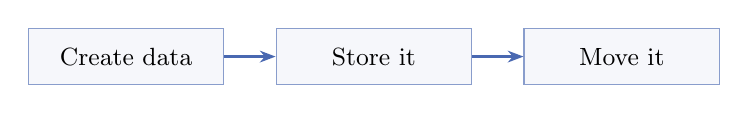
\begin{tikzpicture}[node distance=0.65cm]
      \node[stage,text width=2.25cm] (data) {Create data};
      \node[stage,text width=2.25cm,right=of data] (store) {Store it};
      \node[stage,text width=2.25cm,right=of store] (move) {Move it};
      \draw[link] (data)--(store); \draw[link] (store)--(move);
    \end{tikzpicture}
  \end{center}
  \small Compression reduces the bytes we must store and transmit.
  \credit{Source: \href{https://www.itu.int/itu-d/reports/statistics/wp-content/uploads/sites/5/2026/11/ITUFactsAndFigures2026.pdf}{ITU, Facts and Figures 2026, p. 16}. Traffic growth is a connectivity indicator, not total data creation.}
  \note{Compression matters because recording, storage and communication all consume resources. The ITU reports 18.2 percent average annual growth in mobile broadband traffic since 2021. Its 2026 estimate is 1.7 zettabytes. These figures describe network traffic, not the entire amount of data created worldwide. LLMs and robots give intuitive examples of systems that handle multiple data types. The question becomes more delicate when the data are brain recordings.}
\end{frame}

% Slide 2: all technique families from the website.
\begin{frame}[t]{Compression across modalities}
  \begin{columns}[T,onlytextwidth]
    \column{0.46\textwidth}
      \textbf{Recover every value}\par\medskip
      \textcolor{eegblue}{Huffman coding}\\
      \small Frequent symbols get shorter codes.\par\medskip
      \normalsize\textcolor{eegblue}{ZIP / DEFLATE}\\
      \small Repeated strings + Huffman coding.\par\medskip
      \normalsize\textcolor{eegblue}{PNG}\\
      \small Pixel prediction + lossless coding.
    \column{0.49\textwidth}
      \textbf{Allow some information loss}\par\medskip
      \textcolor{eegcoral}{MP3}\\
      \small Spend bits using a hearing model.\par\smallskip
      \normalsize\textcolor{eegcoral}{Uniform / $\mu$-law quantization}\\
      \small Fewer amplitude levels.\par\smallskip
      \normalsize\textcolor{eegcoral}{JPEG}\\
      \small Transform + quantize image detail.\par\smallskip
      \normalsize\textcolor{eegcoral}{Thresholding / dithering}\\
      \small Reduce pixel precision; retain tone differently.
  \end{columns}
  \vfill
  \small\alert{Quantization discards precision. Entropy coding packs what remains.}
  \credit{Background: \href{https://www.rfc-editor.org/rfc/rfc1951}{Deutsch, RFC 1951 (1996)}; project Techniques module. Thresholding and dithering are precision-reduction steps, not complete file formats.}
  \note{These are the technique families in the website. Huffman coding and ZIP are general-purpose lossless ideas; PNG applies lossless coding to images. DEFLATE combines LZ77 string matching with Huffman coding. MP3 is perceptual audio coding, not an EEG compressor. Mu-law companding is invertible before quantization: the loss comes from subsequently using finitely many levels. PNG is lossless; JPEG is normally lossy. Thresholding and dithering can map grayscale to one bit per pixel; bit packing and file coding are still needed to store it compactly.}
\end{frame}

% Slide 3: a licensed illustration plus a technical acquisition diagram.
\begin{frame}[t]{Neural signal capture: EEG}
  \begin{columns}[c,onlytextwidth]
    \column{0.35\textwidth}
      \centering
\includegraphics[width=0.95\linewidth]{images/eeg-cap.png}
    \column{0.60\textwidth}
      \large Electrodes measure\par
      \alert{voltage differences}\par\medskip
      \normalsize One time series per channel.\par\medskip
      Population-level activity, mixed with noise and artifacts.
  \end{columns}
  \vspace{0.45cm}
  \begin{center}
    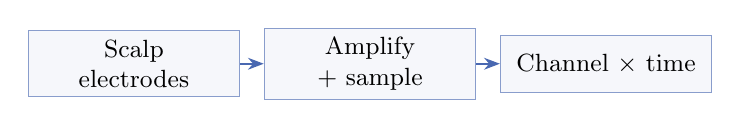
\begin{tikzpicture}[node distance=0.3cm]
      \node[stage,text width=2.45cm] (electrode) {Scalp\\electrodes};
      \node[stage,text width=2.45cm,right=of electrode] (adc) {Amplify + sample};
      \node[stage,text width=2.45cm,right=of adc] (samples) {Channel $\times$ time};
      \draw[link] (electrode)--(adc); \draw[link] (adc)--(samples);
    \end{tikzpicture}
  \end{center}
  \small Time and frequency views reveal different signal features.
  \credit{Acquisition context: \href{https://doi.org/10.1093/gigascience/giz002}{Lee et al. (2019)}. EEG-cap icon: \href{https://commons.wikimedia.org/wiki/File:EEG_Cap_-_The_Noun_Project.svg}{CIV / The Noun Project, CC0}. Illustration is not our apparatus.}
  \note{EEG is non-invasive scalp recording. Each channel measures voltage relative to another location or reference; it is not an isolated neuron's output or a direct reading of thoughts. Amplification, filtering and analog-to-digital conversion produce sampled multichannel time series. Scalp position and reference affect the measurements. Frequency content, changes across channels and responses aligned to stimuli provide different analysis features. The icon is a generic illustration, not a photograph of OpenBMI participants or equipment.}
\end{frame}

% Slide 4: explicit illustrative arithmetic, not a measured study result.
\begin{frame}[t]{Why EEG needs compression}
  \begin{center}
    \large Many channels $\times$ continuous recording
    \vspace{0.4cm}

    {\large $64\times256\times16\times86\,400\,/\,8$}\par
    \small channels\quad samples/s\quad bits/sample\quad seconds/day
    \vspace{0.35cm}

    {\fontsize{27}{31}\selectfont\color{eegteal}2.83 GB per day}
  \end{center}
  \vspace{0.35cm}
  \begin{columns}[T,onlytextwidth]
    \column{0.30\textwidth}\centering\textbf{Storage}\\\small Long recordings accumulate.
    \column{0.32\textwidth}\centering\textbf{Wireless links}\\\small Bandwidth is limited.
    \column{0.31\textwidth}\centering\textbf{Wearable devices}\\\small Sending bits costs energy.
  \end{columns}
  \credit{Illustrative raw 16-bit recording; decimal GB, metadata excluded. Context: \href{https://doi.org/10.1109/ATC.2015.7388309}{Dao et al. (2015)} and \href{https://doi.org/10.3390/info13040186}{Zhang et al. (2022)}. Our benchmark uses a different 12-channel, float32 representation.}
  \note{This is arithmetic, not a measured recording size or a reported compression ratio: 64 channels times 256 samples per second times 16 bits times 86,400 seconds divided by eight equals 2,831,155,200 bytes. Larger montages and longer recordings scale the burden. For wireless wearable EEG, communication can also constrain bandwidth and energy. We did not measure battery savings or device energy. Our benchmark stores twelve channels at 128 Hz in float32, so the later storage allowances use a separate, explicitly defined baseline.}
\end{frame}

% Slide 6: representative classical work; no cross-paper leaderboard.
\begin{frame}[t]{Lossless and lossy EEG compression}
  \textbf{Lossless: recover the original samples}\par\smallskip
  \begin{center}
    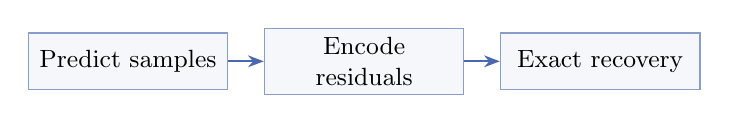
\begin{tikzpicture}[node distance=0.45cm]
      \node[stage,text width=2.3cm] (predict) {Predict samples};
      \node[stage,text width=2.3cm,right=of predict] (residual) {Encode residuals};
      \node[stage,text width=2.3cm,right=of residual] (exact) {Exact recovery};
      \draw[link] (predict)--(residual);\draw[link] (residual)--(exact);
    \end{tikzpicture}
  \end{center}
  \small Memon et al. (1999): context-based lossless / near-lossless coding.
  \vspace{0.4cm}

  \normalsize\textbf{Lossy: trade precision for fewer bytes}\par\smallskip
  \begin{center}
    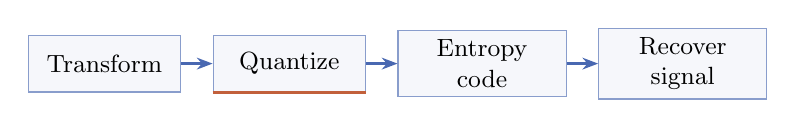
\begin{tikzpicture}[node distance=0.4cm]
      \node[stage,text width=1.7cm] (transform) {Transform};
      \node[stage,text width=1.7cm,right=of transform] (quantize) {Quantize};
      \node[stage,text width=1.9cm,right=of quantize] (code) {Entropy code};
      \node[stage,text width=1.9cm,right=of code] (recover) {Recover\\signal};
      \draw[link] (transform)--(quantize);\draw[link] (quantize)--(code);
      \draw[link] (code)--(recover);
      \draw[eegcoral,very thick] (quantize.south west)--(quantize.south east);
    \end{tikzpicture}
  \end{center}
  \small Higgins et al. (2013): wavelet coefficient quantization / thresholding.\par\smallskip
  Dao et al. (2015): classical methods and storage--distortion trade-offs.\par
  \vspace{0.25cm}
  \small\alert{Smaller file size and smaller waveform error are different goals.}
  \credit{\href{https://doi.org/10.1109/4233.788586}{Memon et al., 1999};
    \href{https://doi.org/10.1016/j.compbiomed.2013.02.011}{Higgins et al., 2013};
    \href{https://doi.org/10.1109/ATC.2015.7388309}{Dao et al., 2015}. Diagrams summarize method families, not a reproduction of any paper.}
  \note{Lossless predictors exploit repeated or predictable structure and encode what the predictor missed, without discarding sample values. Near-lossless coding permits bounded error. Transform-based lossy methods instead represent the waveform using coefficients and reduce their precision or discard some. Higgins studies quantization and thresholding within wavelet compression; our experiment uses a simpler DCT method, not their wavelet codec. Dao provides a survey and motivates compression ratio and waveform-distortion measures. Compression ratio is original bytes divided by stored bytes. PRD and NRMSE depend on the chosen normalization, so papers with different definitions or raw sample precision are not directly comparable. We do not put their compression ratios on a common performance leaderboard.}
\end{frame}

% Slide 7: connect task-aware literature to a fixed-reader comparison.
\begin{frame}[t]{Task-preserving EEG compression}
  \begin{center}
    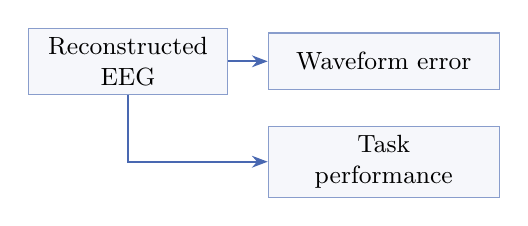
\begin{tikzpicture}[node distance=0.5cm]
      \node[stage,text width=2.3cm] (signal) {Reconstructed EEG};
      \node[stage,text width=2.7cm,right=of signal] (error) {Waveform error};
      \node[stage,text width=2.7cm,below=0.45cm of error] (task) {Task\\performance};
      \draw[link] (signal.east)--(error.west);
      \draw[link] (signal.south)|-(task.west);
    \end{tikzpicture}
  \end{center}
  \small
  \textbf{Zhang et al. (2022)}\quad Personalized SSVEP compression; test recognition.\par\medskip
  \textbf{Strypsteen \& Bertrand (2023)}\quad Jointly learn coding and inference.\par\medskip
  \textbf{Carzaniga et al. (2025)}\quad Learned codec; reconstruction and task evaluations.\par
  \vspace{0.35cm}
  \normalsize\alert{Our comparison keeps the reader fixed after calibration.}
  \credit{\href{https://doi.org/10.3390/info13040186}{Zhang et al., Information 2022};
    \href{https://homes.esat.kuleuven.be/~abertran/reports/Strypsteen_ICASSP2023.pdf}{Strypsteen \& Bertrand, ICASSP 2023};
    \href{https://proceedings.iclr.cc/paper_files/paper/2025/file/28c9ce39a89c03f0bdd9725907d5abbc-Paper-Conference.pdf}{Carzaniga et al., ICLR 2025}.}
  \note{Preserving downstream recognition after compression is established work, not a novelty claim for this project. Zhang and colleagues combine DCT, personalized neural reconstruction and nonuniform quantization, and evaluate SSVEP recognition after reconstruction. Strypsteen and Bertrand jointly optimize source coding and an inference network for motor execution in an emulated wireless sensor network; this is not the same motor-imagery task used here. BrainCodec studies learned EEG/iEEG compression, including downstream and expert evaluations. Our narrower question asks how several simple compressors affect three tasks when the existing original-data reader remains frozen. We do not reproduce these neural codecs or claim to outperform them.}
\end{frame}

% Slide 7: central question and the distinct information each task uses.
\begin{frame}[t]{Our central question}
  \vspace{0.35cm}
  \begin{center}
    \Large At the same storage allowance,\\[0.15cm]
    \alert{which EEG tasks lose performance fastest?}
  \end{center}
  \vspace{0.6cm}
  \begin{columns}[T,onlytextwidth]
    \column{0.31\textwidth}\centering
      \textcolor{eegteal}{\Large SSVEP}\par\medskip
      Which flickering target?\par\smallskip
      \small A sustained rhythm
    \column{0.32\textwidth}\centering
      \textcolor{eegcoral}{\Large Motor imagery}\par\medskip
      Left or right hand?\par\smallskip
      \small A spatial power pattern
    \column{0.30\textwidth}\centering
      \textcolor{eegblue}{\Large P300}\par\medskip
      Target or non-target?\par\smallskip
      \small A brief event response
  \end{columns}
  \vfill
  \begin{center}\small Does the answer survive a change of compressor or reader?\end{center}
  \credit{Motivation: different tasks use different features. This is a controlled comparison of task--reader pipelines, not a proposed universal ranking.}
  \note{We chose three broad paradigms rather than several variants of one task. SSVEP identifies one of four visual flicker targets. Motor imagery distinguishes imagined left/right hand movements. P300 detects a target flash using the brief response after a stimulus; this is single-flash detection, not complete spelling accuracy. Different features may react differently to quantization or removal of frequency components. Comparing the same people and stored montage reduces confounds, while baseline difficulty and decoder design still differ.}
\end{frame}

% Slide 8: the full setup, with technical details in presenter notes.
\begin{frame}[t]{Experimental setup}
  \small\textbf{20 new people}\quad 3 tasks\quad 12 channels\quad 128 samples/s
  \vspace{0.25cm}
  \begin{center}
    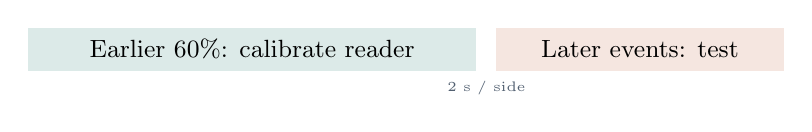
\begin{tikzpicture}
      \fill[eegteal!16] (0,0) rectangle (5.7,0.55);
      \fill[eegcoral!16] (5.95,0) rectangle (9.6,0.55);
      \node[font=\small] at (2.85,0.275) {Earlier 60\%: calibrate reader};
      \node[font=\small] at (7.775,0.275) {Later events: test};
      \node[font=\tiny,muted,below] at (5.825,0) {2 s / side};
    \end{tikzpicture}
  \end{center}
  \vspace{0.1cm}
  \begin{center}
    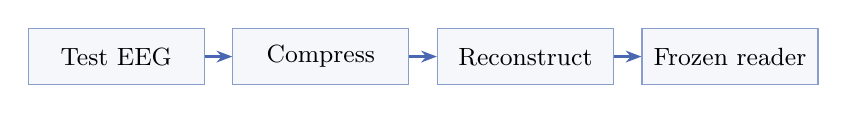
\begin{tikzpicture}[node distance=0.35cm]
      \node[stage,text width=2.0cm] (input) {Test EEG};
      \node[stage,text width=2.0cm,right=of input] (codec) {Compress};
      \node[stage,text width=2.0cm,right=of codec] (restore) {Reconstruct};
      \node[stage,text width=2.0cm,right=of restore] (reader) {Frozen reader};
      \draw[link] (input)--(codec);\draw[link] (codec)--(restore);\draw[link] (restore)--(reader);
    \end{tikzpicture}
  \end{center}
  \smalltext{Uniform, $\mu$-law or DCT; each followed by bit packing and ZIP.}
  \medskip
  \centering
  {\fontsize{8.5}{10.5}\selectfont
  \begin{tabular}{@{}lll r@{}}
    \toprule
    Task & Primary reader & Alternative & Original BA\\
    \midrule
    SSVEP & CCA & Spectral peaks & \BaselineSSVEP\%\\
    Motor imagery & CSP + LDA & Band power + LDA & \BaselineMI\%\\
    P300 & Time bins + LDA & Logistic regression & \BaselineERP\%\\
    \bottomrule
  \end{tabular}}\par
  \medskip
  \smalltext{Caps: \textbf{32 / 64 / 128 / 256 B/s/channel}, including reconstruction metadata.}
  \smalltext{Score loss = original $-$ reconstructed balanced accuracy (percentage points).}
  \credit{\href{https://doi.org/10.1093/gigascience/giz002}{OpenBMI, Lee et al. (2019)}; first recording day only. Pilot: 4 people, kept separate; development: 2, excluded from means.}
  \note{Evaluation subjects are S07--S26, selected in advance. S03--S06 remain the separate pilot and S01--S02 are development checks. The input has the same twelve channels for every task. Continuous recordings are resampled to 128 Hz and filtered from 0.5 to 40 Hz. The split is chronological at 60 percent of events. Training epochs finish two seconds before the boundary, and test epochs begin two seconds after it. Filtering is offline and noncausal, which remains a limitation. SSVEP and MI epochs last four seconds; P300 epochs last one second. Overlapping P300 test epochs share a single encoded continuous recording. One-second codec frames choose the least waveform MSE among a predefined candidate grid that fits each cap, without labels or classifier outcomes. Models and event annotations are outside EEG payload for every method. Raw selected float32 requires 512 bytes/s/channel. Balanced accuracy averages recall across classes; chance is 25 percent for SSVEP and 50 percent for MI/P300. Each person's score receives equal weight. CCA uses known frequency templates. CSP is a learned spatial filter; LDA is linear discriminant analysis. Alternative readers are fixed in advance, calibrated on original early data and never adapted to compression. Both P300 readers share the same low-frequency time-bin features. A float32+ZIP control must recover exact samples and preserve predictions.}
\end{frame}

% Slide 9: native vector plots and a native table from verified exports.
\begin{frame}[t]{Storage allowance and recognition loss}
  \smalltext{Primary readers: mean loss across 20 new participants}
  {\centering
    \begin{tikzpicture}
      \begin{groupplot}[
        group style={group size=3 by 1,horizontal sep=0.33cm},
        scale only axis,width=3.0cm,height=2.15cm,
        xmin=29,xmax=282,xmode=log,log basis x=2,
        xtick={32,64,128,256},xticklabels={32,64,128,256},
        ymin=-3,ymax=22,ytick={0,10,20},
        tick label style={font=\fontsize{7}{8}\selectfont},
        title style={font=\small},label style={font=\scriptsize},
        grid=major,grid style={gray!15},axis line style={gray!45},
        legend style={draw=none,font=\scriptsize,legend columns=3}]
        \nextgroupplot[title={Uniform + ZIP},ylabel={Loss (pp)}]
          \taskcurve{SSVEP}{eegteal}{uniform}
          \taskcurve{MI}{eegcoral}{uniform}
          \taskcurve{ERP}{eegblue}{uniform}
        \nextgroupplot[title={$\mu$-law + ZIP},yticklabels=\empty]
          \taskcurve{SSVEP}{eegteal}{mulaw}
          \taskcurve{MI}{eegcoral}{mulaw}
          \taskcurve{ERP}{eegblue}{mulaw}
        \nextgroupplot[title={DCT + ZIP},yticklabels=\empty]
          \taskcurve{SSVEP}{eegteal}{dct}
          \taskcurve{MI}{eegcoral}{dct}
          \taskcurve{ERP}{eegblue}{dct}
      \end{groupplot}
    \end{tikzpicture}\par
    \smalltext{\textcolor{eegteal}{SSVEP}\qquad\textcolor{eegcoral}{Motor imagery}\qquad\textcolor{eegblue}{P300}}
    \smalltext{Storage allowance (B/s/channel); shading: pointwise 95\% intervals.}
  }\smallskip
  \smalltext{At 32 B/s/channel: \textcolor{eegteal}{primary} / \textcolor{eegcoral}{alternative} reader loss (pp)}
  {\centering{\fontsize{8.5}{10.5}\selectfont
\begin{tabular}{lrrr}
\toprule
Task & Uniform & $\mu$-law & DCT\\
\midrule
SSVEP & \textcolor{eegteal}{12.13} / \textcolor{eegcoral}{4.92} & \textcolor{eegteal}{12.95} / \textcolor{eegcoral}{7.58} & \textcolor{eegteal}{8.82} / \textcolor{eegcoral}{10.88}\\
Motor imagery & \textcolor{eegteal}{9.22} / \textcolor{eegcoral}{8.44} & \textcolor{eegteal}{10.91} / \textcolor{eegcoral}{7.75} & \textcolor{eegteal}{4.10} / \textcolor{eegcoral}{7.46}\\
P300 & \textcolor{eegteal}{9.47} / \textcolor{eegcoral}{12.30} & \textcolor{eegteal}{9.60} / \textcolor{eegcoral}{12.25} & \textcolor{eegteal}{0.61} / \textcolor{eegcoral}{2.25}\\
\bottomrule
\end{tabular}}
\par}
  \credit{Measured exports: results/benchmark and results/robustness. Bootstrap: 10,000 resamples of whole participants, all conditions paired. Lines join tested settings only.}
  \note{These are measured observations, not simulated curves. Lower loss is better; negative loss means a slightly higher reconstructed-data score. At the tightest cap the primary readers put SSVEP highest for every method. The alternative readers put P300 highest for uniform and mu-law, and SSVEP highest for DCT. The original baselines differ between readers, so this is sensitivity to the readout, not a contest to declare one universally better. Intervals are pointwise percentile intervals from participant-level resampling, not trial-level intervals or multiplicity-adjusted tests. Equal caps do not produce exactly equal achieved rates; those rates are exported on the site. Three primary motor-imagery baselines are weak and remain included. The four-person pilot's uniform and mu-law task ordering does not repeat in the larger primary cohort.}
\end{frame}

% Slide 10: emphasize the strongest repeated local result and the uncertainty.
\begin{frame}[t]{Summary and findings}
  \begin{columns}[T,onlytextwidth]
    \column{0.43\textwidth}
      \textbf{The reader changes the ordering.}\par\medskip
      Primary SSVEP vs MI:\\no clear separation at the tightest cap.\par\medskip
      \alert{P300 + DCT repeats across both readers and all 20 people.}
    \column{0.54\textwidth}
      \smalltext{P300: fewer points lost with DCT than uniform}
      \begin{tikzpicture}
        \begin{axis}[width=5.9cm,height=3.6cm,
          xmin=0,xmax=12.5,ymin=-0.6,ymax=1.6,
          ytick={0,1},yticklabels={Alternative,Primary},
          xtick={0,5,10},xlabel={Advantage (pp)},
          tick label style={font=\scriptsize},label style={font=\scriptsize},
          axis line style={gray!40},xmajorgrids,grid style={gray!15}]
          \addplot[only marks,mark=*,mark size=2.4pt,color=eegteal,
            error bars/.cd,x dir=both,x explicit]
            table[x=mean,y=row,x error minus=minus,x error plus=plus,col sep=comma]{data/p300-advantage.csv};
        \end{axis}
      \end{tikzpicture}
      \smalltext{\PrimaryAdvantage\ pp / \AlternativeAdvantage\ pp\par
        Paired means; 95\% intervals.}
  \end{columns}
  \vspace{0.4cm}
  \small\textbf{A close waveform, a similar score and identical decisions are different promises.}
  \credit{32 B/s/channel. Both P300 readers use the same low-frequency features. These results describe the tested pipelines, not an intrinsic or clinical ranking of EEG tasks.}
  \note{At 32 bytes/s/channel, primary mean losses are 12.13/9.22/9.47 pp for uniform, 12.95/10.91/9.60 for mu-law, and 8.82/4.10/0.61 for DCT, ordered SSVEP/MI/P300. All primary SSVEP-minus-MI paired intervals cross zero at this cap. SSVEP is the largest-loss task for only eight of twenty people under uniform, despite its largest group mean. Changing readers changes the task ordering. The strongest repeated local result is P300's DCT advantage over uniform: 8.87 pp with interval 7.95--9.83 for the primary reader, and 10.05 pp with interval 9.00--11.20 for the alternative. Every new participant shows that direction. Both P300 readers use the same low-frequency features, so this does not test all P300 analysis methods. P300 DCT changes about 5.9 percent of primary predictions despite only 0.61 pp mean score loss; correct-to-incorrect and incorrect-to-correct changes can partly cancel. Baseline difficulty matters: primary SSVEP still scores about 81 percent under tight-cap uniform while MI is about 61 percent against a 50 percent chance level.}
\end{frame}

% Slide 11: limitations are tied to concrete next experiments.
\begin{frame}[t]{Limitations and future work}
  \begin{columns}[T,onlytextwidth]
    \column{0.46\textwidth}
      \textbf{What limits this study?}\par\medskip
      20 new people, one acquisition study.\par\medskip
      One recording day; offline filtering.\par\medskip
      Two readers per task; shared P300 features.\par\medskip
      Simple codecs; equal caps, different actual sizes.
    \column{0.48\textwidth}
      \textbf{What should come next?}\par\medskip
      More datasets and task families.\par\medskip
      More features, readers and EEG codecs.\par\medskip
      Match achieved storage rates more closely.\par\medskip
      Measure streaming latency and device energy.
  \end{columns}
  \vspace{0.55cm}
  \large\alert{Preserve the information needed for the intended use.}
  \credit{The benchmark does not establish a universal task ranking or clinical safety. More data alone cannot remove decoder and feature-design differences.}
  \note{The extension improves the sample size but still uses a fixed, nonrandom subset of one acquisition study. We have not tested a new day, real-time deployment, clinical interpretation or device power. The continuous noncausal filter can couple neighboring samples across the split despite the epoch guard. Original task difficulty differs, and weak baselines are retained. Each task has only two chosen readers. The alternative P300 reader changes the classifier but not the features, so a broader feature comparison is still needed. All codec settings were selected using waveform MSE, not task labels, but their search grids differ. Equal maximum byte caps leave different unused space. Future work should test more datasets and tasks, independently varied feature extractors, stronger EEG codecs and more closely matched achieved rates. Streaming and hardware experiments would be needed for latency or battery claims.}
\end{frame}

% Slide 12: selected linked references. Full BibTeX metadata is in ref.bib.
\begin{frame}[t]{References}
  \begin{columns}[T,onlytextwidth]
    \column{0.48\textwidth}
      \fontsize{8}{9.5}\selectfont
      \refentry{ITU (2026)}{Facts and Figures, p. 16.}
        {https://www.itu.int/itu-d/reports/statistics/wp-content/uploads/sites/5/2026/11/ITUFactsAndFigures2026.pdf}
      \refentry{Deutsch (1996)}{DEFLATE format specification. RFC 1951.}
        {https://www.rfc-editor.org/rfc/rfc1951}
      \refentry{Memon, Kong \& Cinkler (1999)}{Context-based lossless and near-lossless EEG compression.}
        {https://doi.org/10.1109/4233.788586}
      \refentry{Higgins et al. (2013)}{Wavelet coefficient quantization in EEG compression.}
        {https://doi.org/10.1016/j.compbiomed.2013.02.011}
      \refentry{Dao, Li \& Do (2015)}{Lossy Compression Techniques for EEG Signals.}
        {https://doi.org/10.1109/ATC.2015.7388309}
    \column{0.48\textwidth}
      \fontsize{8}{9.5}\selectfont
      \refentry{Zhang et al. (2022)}{Personalized SSVEP EEG compression. Information 13, 186.}
        {https://doi.org/10.3390/info13040186}
      \refentry{Strypsteen \& Bertrand (2023)}{Neural source coding for wireless brain--computer interfacing. ICASSP.}
        {https://homes.esat.kuleuven.be/~abertran/reports/Strypsteen_ICASSP2023.pdf}
      \refentry{Carzaniga et al. (2025)}{The Case for Cleaner Biosignals (BrainCodec). ICLR.}
        {https://proceedings.iclr.cc/paper_files/paper/2025/file/28c9ce39a89c03f0bdd9725907d5abbc-Paper-Conference.pdf}
      \refentry{Lee et al. (2019)}{OpenBMI: EEG dataset for three BCI paradigms. GigaScience 8, giz002.}
        {https://doi.org/10.1093/gigascience/giz002}
  \end{columns}
  \vfill
  \small\textbf{Project website, demonstrations and measured results}\par\smallskip
  \fontsize{7.8}{9.5}\selectfont
  \url{https://da3021-compression-lab-deb044.solidflask.chatgpt.site/}\par\medskip
  \small\href{https://github.com/Deb044/DataCompression}{github.com/Deb044/DataCompression}
  \note{These are selected references supporting the narrative, not an exhaustive systematic review. The full bibliography is in ref.bib. Paper-specific compression ratios are intentionally not compared because recordings, precision, metadata accounting, allowed distortion and downstream models differ. All experimental values in this presentation are from this repository's first-day extension and verified exports. The website links the full measurements, individual predictions, uncertainty intervals, protocol and implementation. Image credits: IIT Guwahati logo from its official website; generic EEG-cap icon by CIV / The Noun Project, public domain under CC0 via Wikimedia Commons.}
\end{frame}

\end{document}
